\documentclass{book}

\usepackage[shortsuper,hacm,ltfont]{common/uruwi}

\newcommand{\lname}{Middle Rymakonian}

\title{lek-\bs{}tsaro-ma sil lek-ma sil se\^otxe-\bs{}ri\^umako}
\author{uruwi}

\begin{document}

\pagecolor{Thistle!25}

\begin{titlepage}
    \makeatletter
    \begin{center}
        {\color{Orchid} \hprule \vspace{1.5ex} \\}
        {\Huge \ltfont \textcolor{Plum}{LKe\bs{}TSxaRMoa SL LKeMa SL STfXe\bs{}RMyaKo}\\}
        {\large \kardinal \textcolor{Purple}{\@title} \\}
        {\large \textit{\lname}, the language of \textit{Rymako} \\}
        {\color{Orchid} \hprule \vspace{1.5ex} \\}
        % ----------------------------------------------------------------
        \vspace{1.5cm}
        {\Large\bfseries \@author}\\[5pt]
        %uruwi@protonmail.com\\[14pt]
        % ----------------------------------------------------------------
        \vspace{2cm}
        {\Large\textlt{IVvoQMxeBPieLBxf TXxeKy}} \\
        \textkardinal{f\^ho\^e.on\^g-mebi-pelbe\^o txeki\^u} \\[5pt]
        \emph{A complete grammar}\\[2cm]
        %{in partial fulfilment for the award of the degree of} \\[2cm]
        %\tsc{\Large{{Doctor of Philosophy}}} \\[5pt]
        %{in some subject} \vspace{0.4cm} \\[2cm]
        % {By}\\[5pt] {\Large \sc {Me}}
        \vfill
        % ----------------------------------------------------------------
        %\includegraphics[width=0.19\textwidth]{example-image-a}\\[5pt]
        %{blah}\\[5pt]
        %{blahblah}\\[5pt]
        %{blahblah}\\
        \vfill
        {\@date}
    \end{center}
    \makeatother
\end{titlepage}

\pagecolor{Thistle!15}

\begin{center}
    \textit{Dedicated to Gufferdk.}
\end{center}

\begin{verbatim}
Branch: canon
Version: 0.1
Date: 2017-12-22 (29 dia len)
\end{verbatim}

(C)opyright 2017 Uruwi. See README.md for details.

\tableofcontents

\section{Introduction}

\chapter{Phonology and orthography}

\section{Phoneme inventory}

\lname{} underwent several sound changes from Lek-Tsaro, in the following order:

\begin{alignat*}{2}
  % \alpha &\rightarrow \omega &\quad(\lambda \blacklozenge \rho) &\quad[\Gamma]
  \text{s} &\rightarrow \text{s͎} &\quad(\blacklozenge \{\text{w}, \text{j}, \text{u}, \text{y}\}) &\quad \textit{NB this is a whistled sibiliant.} \\
  \text{ŋ} &\rightarrow \text{ɲ} &\quad(\square \blacklozenge) \\
  \text{θx} &\rightarrow \text{θ} &\quad\lnot(\blacklozenge \square) [\chi = \emptyset] \\
  C_1[+fr] &\rightarrow C_1[+v] &\quad(V_1 \blacklozenge V_2[-hi]) \\
  \text{ɹ} &\rightarrow \text{z} &\quad(V_1 \blacklozenge V_2) \\
  \{\text{y̜}, \text{u̜}\} &\rightarrow \text{ʉ̜} \\
  V_1[+r] &\rightarrow \text{w}V_1[-r] \\
  \text{k} &\rightarrow \text{c} &\quad (\blacklozenge \text{i}) \\
  \text{t} &\rightarrow \text{tʃ} &\quad (\blacklozenge \{\text{i}, \text{ɛ}\}) \\
  \text{r} &\rightarrow \text{ɾ} \\
\end{alignat*}

Thus \lname{} has the following phoneme inventory:

\begin{table}[h]
  \caption{The consonants of \lname.}
  \centering
  \begin{tabular}{l|llllll}
      & Bilabial & Dental & Alveolar & Palatal & Velar & Glottal \\
      \hline
      Nasal & m & & n & ɲ & ŋ & \invalid \\
      Plosive & p b & & t d & c ɟ & k ɡ & ʔ \\
      Fricative & f v & θ ð & s z & ʃ ʒ & x ɣ & \\
      (coärticulated) & fx vɣ & θx ðɣ & & fʃ vʒ & & \invalid \\
      (whistled) & \invalid & \invalid & s͎ z͎ & & \invalid & \invalid \\
      Affricate & & & ts & tʃ & & \\
      Lateral fricative & \invalid & & ɬ ɮ & & & \invalid \\
      Approximant & & & ɹ & j & w & \\
      Lateral approximant & \invalid & & l & & & \invalid \\
      Tap & & & ɾ & & \invalid & \invalid \\
  \end{tabular}
\end{table}

\begin{table}[h]
  \centering
    \caption{The vowels of \lname.}
    \begin{tabular}{l|lll}
        & Front & Central & Back \\
        \hline
        High & i & ʉ̜ & ɯ \\
        Mid & ɛ & & ʌ \\
        Low & & a & \\
    \end{tabular}
\end{table}

In addition to consonants and vowels, \lname{} has rod signals, represented by numbers. Rod A is blue and held by one's dominant hand and B is red and held by one's non-dominant hand.

\begin{enumerate}
    \item Rod A is raised to one's chest, while B is pointed down.
    \item Rods A and B are crossed in the front.
    \item Rod B is raised upwards in front of the nondominant arm, while rod A is lowered.
    \item Rod A is pointed sideways near one's nondominant arm, while rod B is lowered.
    \item Rods A and B are extended to the sides.
    \item Rods A and B are extended, facing forward.
    \item Rod A is raised forward, while B is pointed to the side.
    \item Rod B is raised forward, while A is pointed to the side.
\end{enumerate}

Lowering both rods is interpreted as an absence of a rod signal.

If the use of rods are unavailable, the numerals of the positions may be pronounced.

\section{Hacmisation}

As using IPA is quite wieldly, we shall use the following hacmisation, with superscript letters to indicate phonemes not found in Arka.

\begin{table}[h]
  \caption{The consonants of \lname. \label{table:hcons}}
  \centering
  \begin{tabular}{l|>{\kardinal}l>{\kardinal}l>{\kardinal}l>{\kardinal}l>{\kardinal}l>{\kardinal}l}
      & \textnormal{Bilabial} & \textnormal{Dental} & \textnormal{Alveolar} & \textnormal{Palatal} & \textnormal{Velar} & \textnormal{Glottal} \\
      \hline
      Nasal & m & & n & n\^y & n\^g & \invalid \\
      Plosive & p b & & t d & t\^y d\^y & k g & . \\
      Fricative & f v & s\^f z\^v & s z & x j & k\^x g\^j & \\
      (coärticulated) & f\^h v\^h & s\^h z\^h & & f\^x v\^j & & \invalid \\
      (whistled) & \invalid & \invalid & s\^w z\^w & & \invalid & \invalid \\
      Affricate & & & t\^s & t\^x & & \\
      Lateral fricative & \invalid & & x\^l z\^l & & & \invalid \\
      Approximant & & & r & y & w & \\
      Lateral approximant & \invalid & & l & & & \invalid \\
      Tap & & & c & & \invalid & \invalid \\
  \end{tabular}
\end{table}

\begin{table}[h]
  \centering
    \caption{The vowels of \lname. \label{table:hvows}}
    \begin{tabular}{l|>{\kardinal}l>{\kardinal}l>{\kardinal}l}
        & \textnormal{Front} & \textnormal{Central} & \textnormal{Back} \\
        \hline
        High & i & q & u \\
        Mid & e & & o \\
        Low & & a & \\
    \end{tabular}
\end{table}

Rod signs are represented by the hacm digits \hortho{1 2 3 4 5 6 7 8} attached to the end of the verbs they encompass. Proper words are preceded by a backslash \hortho{\bs{}}.

Note that the hacmisation is slightly different from Lek-Tsaro's use of hacm. Lek-Tsaro's \hortho{h j} are now written using \hortho{k\^x x\^l}, for instance.

\section{Phonotactics}

As opposed to Lek-Tsaro, which uses syllables, \lname{} uses \emph{phonoruns}. The following \emph{defined categories} are used:

\begin{table}[ht]
  \caption{Categories of phonemes. \label{table:phonemecats}}
  \centering
  \begin{tabu} to \linewidth {l|>{\kardinal}X}
      Category & \textnormal{Phonemes} \\
      \hline
      Full-open & a e i o u r v z\^v z z\^w j g\^j z\^l y w 5 6 \\
      Half-open & q r l m n n\^y n\^g s\^l 7 \\
      Neutral & s s\^w x v\^h z\^h v\^j 1 2 \\
      Half-closed & f x k\^x c 8 \\
      Full-closed & s\^f f\^h s\^h f\^x p b t d t\^y d\^y k g t\^s t\^x . 3 4 \\
  \end{tabu}
\end{table}

These are converted into \emph{actual categories} as follows:

\begin{itemize}
  \item Full-open and full-closed phonemes are always realised as open and closed, respectively.
  \item Half-open phonemes are open unless the previous phoneme is full-closed.
  \item Half-closed phonemes are closed unless the previous phoneme is full-open.
  \item Neutral phonemes that do not occur word-initially inherit the actual category of the phoneme before it.
  \item Neutral phonemes that occur word-initially are closed.
\end{itemize}

A \emph{phonorun}, then, is a maximal sequence of phonemes that are either all open or all closed within a word. For instance, take \hortho{s\^h.aen < *s\^ha.en}:

\begin{center}
  \begin{tikzpicture}
  %\tikzset{grow'=left}
  %\tikzset{every tree node/.style={anchor=base east}}
  %\tikzset{execute at begin node=\strut}
  %\tikzset{level distance=100pt,sibling distance=10pt}
  %\Tree [.S [.NP LaTeX ] [.VP [.V is ] [.NP fun ] ] ]
  \Tree [
      .$\omega$
      [.$\rho_c$ [.$fc$ \textkardinal{s\^h} ] [.$fc$ \textkardinal{.} ] ]
      [.$\rho_o$ [.$o$ \textkardinal{a} ] [.$fo$ \textkardinal{e} ] [.$ho$ \textkardinal{n} ] ]
  ]
  \end{tikzpicture}
\end{center}

Note that two phonemes in the word were metathesised when it was derived from Lek-Tsaro. In general, a word with $n$ spoken phonemes cannot have more than $\lceil n/2 \rceil$ phonoruns. Therefore, the following changes are executed in order until an application of one rule reduces the number of phonoruns to an acceptable number, after which the other rules are not executed:

\begin{alignat*}{2}
  % \alpha &\rightarrow \omega &\quad(\lambda \blacklozenge \rho) &\quad[\Gamma]
  X_1[do] X_2[dc] R[do] &\rightarrow X_2 X_1 R \\
  X_1[dc] X_2[do] R[dc] &\rightarrow X_2 X_1 R \\
  X_1[dc] X_2[do] \text{ʔ} X_3[do] &\rightarrow X_1 \text{ʔ} X_2 X_3 \\
  X_1[do] \text{ʔ} X_2[do] X_3[dc] &\rightarrow X_1 X_2 \text{ʔ} X_3 \\
  X_1[op \ge 0] X_2[dc] X_3[do] X_4[op \le 0] &\rightarrow X_1 X_3 X_2 X_4 &\quad[X_1.op + X_3.op - X_2.op - X_4.op \ge 6] \\
  X_1[op \le 0] X_2[do] X_3[dc] X_4[op \ge 0] &\rightarrow X_1 X_3 X_2 X_4 &\quad[X_2.op + X_4.op - X_1.op - X_3.op \ge 6] \\
  X_1[do] X_2[dc] X_3[do] &\rightarrow X_1 X_3 X_2 &\quad\text{for ever} \\
  X_1[dc] X_2[do] X_3[dc] &\rightarrow X_2 X_1 X_3 &\quad\text{for ever} \\
\end{alignat*}

where $R$ means a rod signal and $op$ stands for \emph{openness} (full-open = $2$, neutral = $0$, full-closed = $-2$). $do$ is short for $op > 0$, and $dc$ is short for $op < 0$. 

All of the rules above move from right to left and do not occur across compound boundaries. The last two rules are executed alternately in a loop until the number of phonoruns is reduced to an acceptable number or both rules converge to a fixed point. This process will hereafter be called \emph{phonorun reduction}.

In the example above, \hortho{*s\^ha.en} had $4 > \lceil 5 / 2 \rceil$ phonoruns, so the third rule was applied. This changed the word into \hortho{s\^h.aen}, which has $2 \le \lceil 5 / 2 \rceil$ phonoruns.

The dictionary lists forms of roots \emph{before} the phonorun reduction happens, because affixes can radically affect which phonemes are switched.

\section{Vowel harmony}

\lname{} inherits vowel harmony from Lek-Tsaro. Thus \hortho{i e} are front vowels, \hortho{u o} are back vowels and \hortho{a q} are neutral. A root with neither front nor back vowels acts as if it has front vowels. Many affixes will change depending on which vowels are present.

If by some odd chance a word has both front and back vowels, then the rightmost vowel (before phonorun reduction) takes precedence.

\chapter{Syntax}

\section{Basic word order}

The basic word order is VSO. Descriptors follow what they modify.

However, unlike Lek-Tsaro, \lname{} has oblique arguments. As these were historically formed from a preclause, all obliques precede V. Likewise, any arguments with conjunctions also precede V.

Usually, oblique arguments are prepared by prepositions and fall before what they modify, but if an oblique argument is a conjunctional phrase or governs another oblique argument, it uses a postposition instead and precedes its antecedent.

\section{Questions}

Binary questions have the interrogative polarity marker and no change to syntax.

In wh-questions, the wh-word is pulled to the front (i.~e. before the verb). This requires case marking for the wh-word: \\
~\\
{}[TODO: example] \\

This applies only to questions, not interrogative-mood clauses that act as relative clauses: \\
~\\
{}[TODO: example]

\section{Multiple clauses}

A sentence might have multiple clauses. Each clause in a sentence follows the basic VSO order, and clauses are separated with commas.

\chapter{Nouns}

Nouns are declined for number, case and definiteness.

\section{Number}

Countable nouns come in two numbers: \emph{dual} and \emph{non-dual}.

There are two different conceptualisations of the dual number. Some dialects use the dual number to refer to all cases with two objects (we say that they have the \emph{unpaired dual}); others use it only to refer to objects in pairs (these lack the unpaired dual). In general, dialects without the unpaired dual are more prevalent in cities, as well as northern regions.

Each countable noun has \emph{an inherent number}. A noun whose number agrees with its inherent number receives no marking; a mismatch causes the noun to receive a special affix.

\section{Case}

In a clause with both the subject and object directly expressed in that order, both the subject and object are declined in the nominative case (and their roles are inferred through word order). In a clause where only one is present, or where both are expressed in the opposite order, the subject will receive the nominative case and the object will receive the accusative case.

\section{Noun classes}

There are three overarching groups of noun classes.

\begin{enumerate}
  \item Countable
  \begin{enumerate}
      \item Sentient -- such as humans, AIs, deities.
      \item Non-sentient -- anything else.
  \end{enumerate}
  \item Measurable
  \begin{enumerate}
      \setcounter{enumi}{2}
      \item Measure -- all measurable nouns, especially units of measurement.
  \end{enumerate}
  \item Uncountable
  \begin{enumerate}
      \setcounter{enumi}{3}
      \item Edible -- edible (to humans).
      \item Inedible -- inedible (to humans).
      \item Abstract -- abstract ideas.
  \end{enumerate}
\end{enumerate}

\section{Definiteness}

The definite form of a noun is formed regularly by reduplicating the first syllable (without the coda): \hortho{maza} ``a person'' becomes \hortho{mamaza} ``the person''.

\section{Declension table}

Here, the inflected forms of words are shown both before and after phonorun reduction to illustrate the pattern. The declension patterns for each class is shown, both for roots ending with consonants and those ending with vowels.

Note that noun declensions for countable and measurable respect vowel harmony. For nouns with back vowels, replace the front vowels with the back vowels of the same height and rounding, and vice versa. (Noun declensions for uncountable classes do not respect vowel harmony.)

\subsection{Countable classes}

\newcommand{\overcol}{& \textnormal{Direct \#} & \textnormal{Inverse \#}}
\begin{longtabu}{|r|>{\kardinal}Y|>{\kardinal}Y|}
    \caption{Declensions for countable nouns. \label{table:ndecc}} \\
    
    \hline
    \overcol \\
    \endfirsthead
    
    \hline
    \overcol \\
    \hline
    \endhead
    
    \hline
    \endfoot
    
    \hline
    \endlastfoot
    
    \hline
    \multicolumn{3}{|l|}{\textnormal{Sentient: \hortho{*maza} ``person''}} \\
    \hline
    Nominative & maza (maza) & maza\hliii{l} (mazal) \\
    Accusative & maza\hliii{n} (mazan) & maza\hliii{nal} (mazanal) \\
    \hline
    \multicolumn{3}{|l|}{\textnormal{Sentient: \hortho{*s\^ha.en} ``magician''}} \\
    \hline
    Nominative & s\^ha.e\hliii{n} (s\^h.aen) & s\^ha.e\hliii{l} (s\^h.ael) \\
    Accusative & s\^ha.e\hliii{rin} (s\^ha.erin) & s\^ha.e\hliii{ril} (s\^ha.eril) \\
    \hline
    \multicolumn{3}{|p{\linewidth}|}{(Note that the final consonant is preserved only in the direct nominative form.)} \\
    \hline
    \multicolumn{3}{|l|}{\textnormal{Non-sentient: \hortho{*mqn\^go} ``rabbit''}} \\
    \hline
    Nominative & mqn\^go (mqn\^go) & mqn\^go\hliii{.u} (mqn\^go.u) \\
    Accusative & mqn\^go\hliii{m} (mqn\^gom) & mqn\^go\hliii{fu} (mqn\^gofu) \\
    \hline
    \multicolumn{3}{|l|}{\textnormal{Non-sentient: \hortho{*.imen} ``house''}} \\
    \hline
    Nominative & .ime\hliii{n} (.imen) & .ime\hliii{.i} (.imei.) \\
    Accusative & .ime\hliii{rim} (.imerim) & .imeri\hliii{fi} (.imerifi) \\
\end{longtabu}

\subsection{Measurable and uncountable classes}

\newcommand{\overcolm}{& \textnormal{Direct}}
\begin{longtabu}{|r|>{\kardinal}Y|}
    \caption{Declensions for measurable and uncountable nouns. \label{table:ndecm}} \\
    
    \hline
    \overcolm \\
    \endfirsthead
    
    \hline
    \overcolm \\
    \hline
    \endhead
    
    \hline
    \endfoot
    
    \hline
    \endlastfoot
    
    \hline
    \multicolumn{2}{|l|}{\textnormal{Measure: \hortho{*rqmq} ``day (continuous)''}} \\
    \hline
    Nominative & rqmq (rqmq) \\
    Accusative & rqmq\hliii{n} (rqmqn) \\
    \hline
    \multicolumn{2}{|l|}{\textnormal{Measure: \hortho{*mel} ``volume'' (in expressions such as \hortho{*mel-yqso} ``cupful'')}} \\
    \hline
    Nominative & me\hliii{l} (mel) \\
    Accusative & me\hliii{rin} (merin) \\
    \hline
    \multicolumn{2}{|l|}{\textnormal{Edible: \hortho{*ter.i} ``beef''}} \\
    \hline
    Nominative & ter.i (teri.) \\
    Accusative & ter.i\hliii{n} (terin.) \\
    \hline
    \multicolumn{2}{|l|}{\textnormal{Edible: \hortho{*man} ``rice''}} \\
    \hline
    Nominative & ma\hliii{n} (man) \\
    Accusative & ma\hliii{nin} (manin) \\
    \hline
    \multicolumn{2}{|l|}{\textnormal{Inedible: \hortho{*ruto} ``gold''}} \\
    \hline
    Nominative & ruto (ruot) \\
    Accusative & ruto\hliii{be} (rutboe) \\
    \hline
    \multicolumn{2}{|l|}{\textnormal{Inedible: \hortho{*kacas} ``stone''}} \\
    \hline
    Nominative & kacas (kacas) \\
    Accusative & kacas\hliii{pe} (kacaspe) \\
    \hline
    \multicolumn{2}{|l|}{\textnormal{Abstract: \hortho{*f\^humo} ``empathy''}} \\
    \hline
    Nominative & f\^humo (f\^humo) \\
    Accusative & f\^humo\hliii{n\^g} (f\^humon\^g) \\
    \hline
    \multicolumn{2}{|l|}{\textnormal{Abstract: \hortho{*gis} ``[the number] five''}} \\
    \hline
    Nominative & gis (gis) \\
    Accusative & gis\hliii{in\^g} (gisin\^g) \\
\end{longtabu}

\appendix

\chapter*{Romanisation}

In this text, the romanisation is used only to transcribe names into English. Whenever possible, the hacmisation should be used.

\begin{table}[h]
  \caption{The consonants of \lname.}
  \centering
  \begin{tabular}{l|llllll}
      & Bilabial & Dental & Alveolar & Palatal & Velar & Glottal \\
      \hline
      Nasal & m & & n & ñ & ŋ & \invalid \\
      Plosive & p b & & t d & ť ď & k g & ' \\
      Fricative & f v & þ ð & s z & š ž & h ħ & \\
      (coärticulated) & fh vħ & þh ðħ & & fš vž & & \invalid \\
      (whistled) & \invalid & \invalid & ŝ ẑ & & \invalid & \invalid \\
      Affricate & & & ts & tš & & \\
      Lateral fricative & \invalid & & ṡ ż & & & \invalid \\
      Approximant & & & r & j & w & \\
      Lateral approximant & \invalid & & l & & & \invalid \\
      Tap & & & ř & & \invalid & \invalid \\
  \end{tabular}
\end{table}

\begin{table}[h]
  \centering
    \caption{The vowels of \lname.}
    \begin{tabular}{l|lll}
        & Front & Central & Back \\
        \hline
        High & i & y & u \\
        Mid & e & & o \\
        Low & & a & \\
    \end{tabular}
\end{table}

The digraphs \ortho{fh vħ þh ðħ fš vž ts tš} correspond to coärticulated consonants and affricates. A hyphen can be used if this is not desired.

Rod signs are represented by the Arabic digits \ortho{1 2 3 4 5 6 7 8} attached to the end of the verbs they encompass. Proper words are preceded by a backslash \ortho{\bs{}}.

\ortho{ŋ} should be capitalised as \ortho{Ŋ} only if one can depend on the majuscule glyph appearing like an N with a hook. Otherwise, it should be spelled \ortho{Ng}.

\end{document}